%% progress-report-8-SubmapVisualization+ROSPackage tex file.
%% Completed By Yuyang Rong(rongyy@shanghaitech.edu.cn) and
%% Jianxiong Cai(caijx@shanghaitech.edu.cn)
%%
%% To edit this file, please use indentions with tab size of 2.
%%

%% File name unchanged. This is just a temp file.

\documentclass[conference,compsoc]{IEEEtran}
\usepackage{cite}
\usepackage{listings}
\usepackage{blindtext}
\usepackage{enumitem}
% for coding highlight
\usepackage{graphicx}
\usepackage{subfigure}
\usepackage[colorlinks=true,urlcolor=blue]{hyperref}
\usepackage{amsmath, amsthm, amssymb}
\usepackage{subfloat}
\usepackage{ulem}
\usepackage{float}
\usepackage{indentfirst}
\newcommand{\subparagraph}{}
\begin{document}
\title{
	Computer Vision Course Project Milestone Report\\
	Gambody \\
}


% author names and affiliations
% use a multiple column layout for up to three different
% affiliations
\author{
	\IEEEauthorblockN{Yuyang Rong, Jingyi Huang, Anqi Pang, Jianxiong Cai, Ziyue Li}
	\IEEEauthorblockA{
		School of Information Science and Technology \\
		ShanghaiTech University \\
	}
}

\maketitle

\begin{abstract}
	In this report we will mark some achievements we have accomplished, and further purpose some problems(along with solutions, maybe) we need to solve in order to reach our goal.
%	In this milestone report we are going to propose the problems we want to solve aiming at our goal of implementing the visual game Gambody. 
	We will specify our technical approach too.
%	We will specify the technical approach we are using at present and what we have achieved so far. The remaining milestones including the dates and sub-goals will be given furthermore.
\end{abstract}
\section{Introduction}
	\par
		We found a popular game called \textit{Hole in the Wall}. In this game one (or two) player(s) are facing a moving wall with a certain shape of hole, the player have to make a specific pose to pass the moving wall or he will be pushed into a water pool behind him.
		Such game is interesting but householders can never have the privilege to play in family gatherings or parties since one can hardly find a moving wall nor adequate safety measurements.
		\begin{figure}[h]
			\centering
			
\includegraphics[width=0.8\linewidth]{./Pic/HIW_Logo}
			\caption{Game Logo}
		\end{figure}
		\begin{figure}[h]
			\centering
			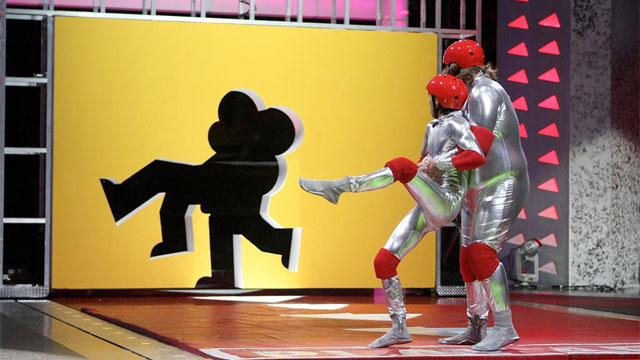
\includegraphics[width=0.45\linewidth]{./Pic/HIW_RedTeam}
			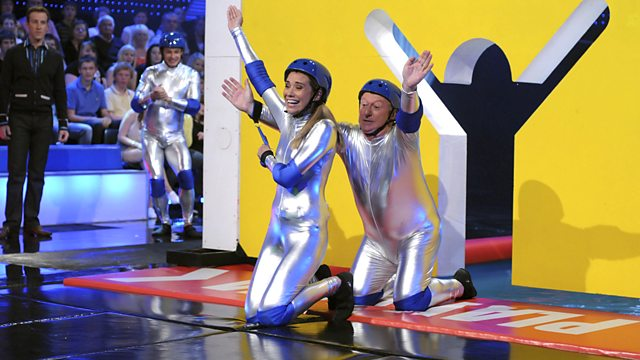
\includegraphics[width=0.45\linewidth]{./Pic/HIW_BlueTeam}
			\caption{Two players in the game posing to pass the wall.}
		\end{figure}
	\par

	\par
		To fix this, we are going to implement a system based on camera so that every one can play this game.
		In our work, we will be using one single camera to track person, it will also give player a bounding box (moving wall).
		The box and player's outfit is compared by our system, the return should be a pass (True) or no pass (False).
%\section{Related Work}
% It seems that this part is not required in the milestone report.
% IF have, please fill in
\section{Technical Approach}
\subsection{Getting camera stream}
\par
We make use of the Image Acquisition Toolbox to connect camera device to MATLAB and achieve real-time image processing and displaying. In general, we keep capturing an image from the camera stream, modify the image we received and show on the screen as long as the camera is working.
\par
To be more specific, we first let MATLAB automatically set camera parameters and invoke the camera since the parameters are device dependent. Then a while loop is maintained to implement the primary procedure during the logging time of the camera.
\par
One of the obstacle we are facing now is that we can't add some pause time before the result is showed to the player. But it would be best if we give player some time to wait.
\subsection{Crop out body}
\par
A simple but useful method has been implemented to detect the body. The principle is that given the camera is fixed, the only area has color changing on the image is the body part.
\par
In detail, we take a photo of the background first, then we subtract it by the images containing body. As the result, we would get a image with only the body part.
% TODO, add some image here of raw body here.
\begin{figure}[h]
	\centering
	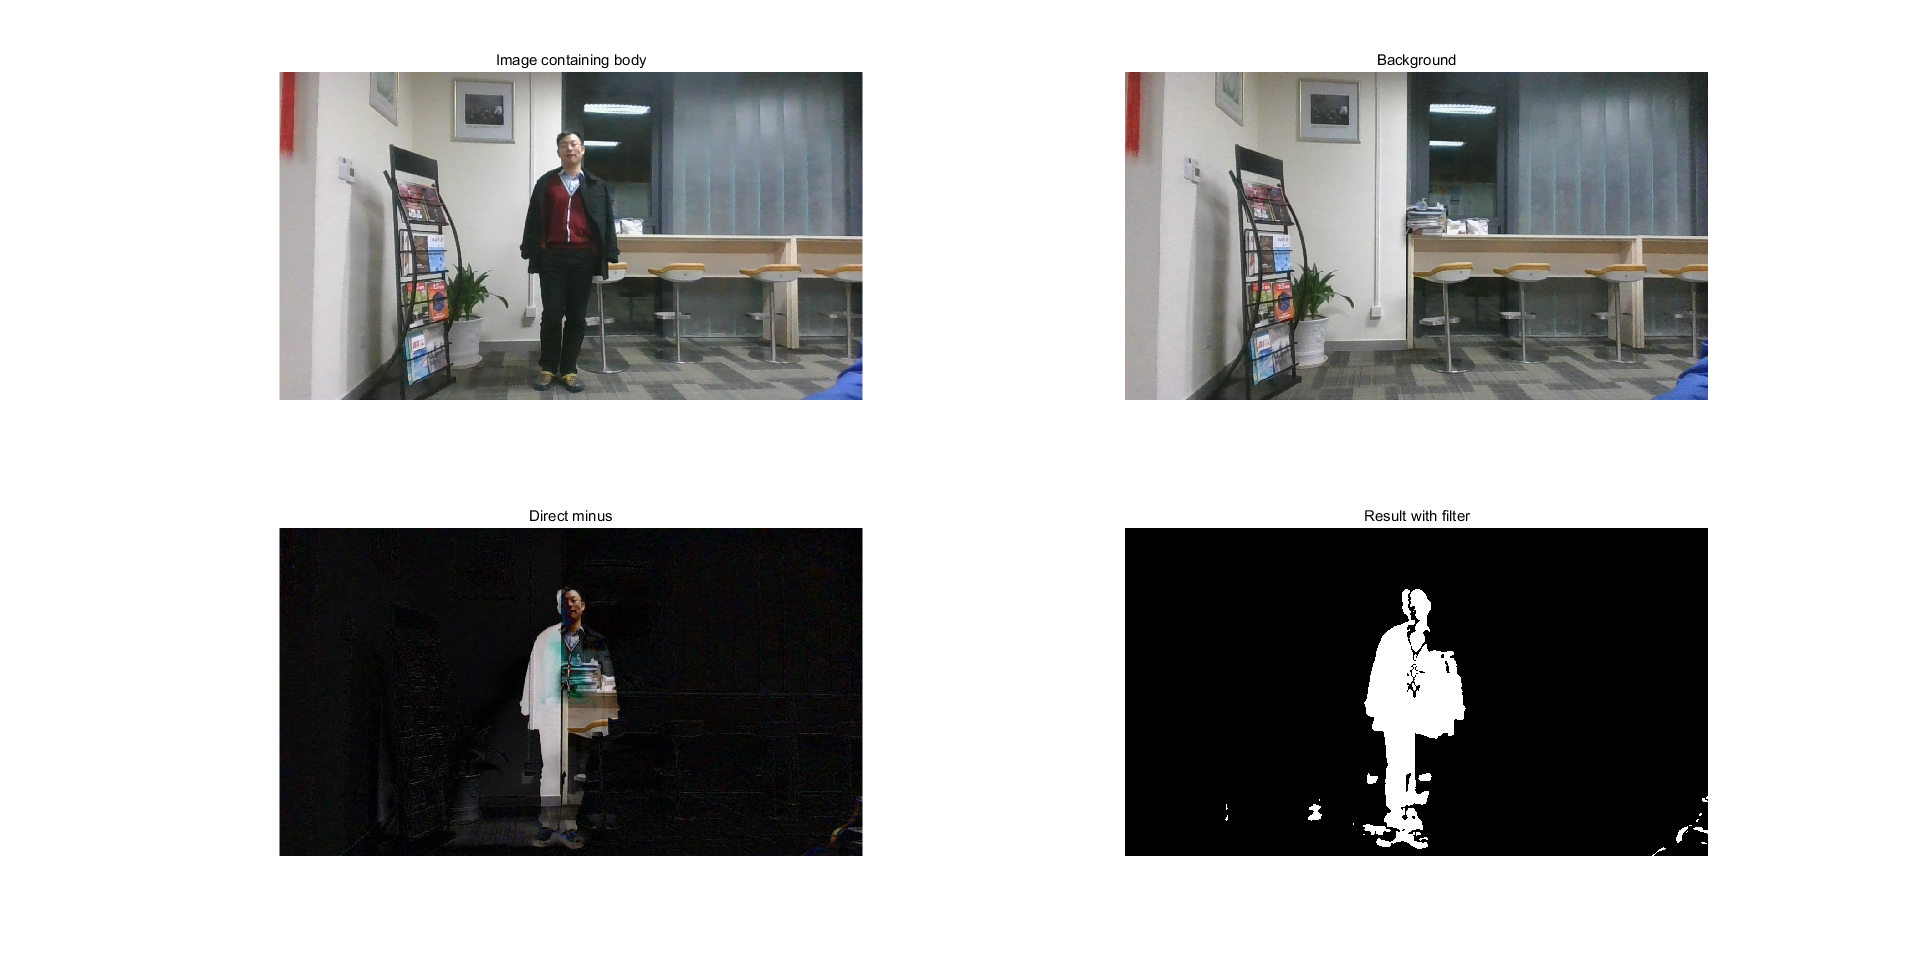
\includegraphics[width=\linewidth]{./Pic/CropBody.png}
	\caption{Upper Left: original photo. Upper Right: Background. Lower Left: the image after subtraction. Lower Right: The body region after we force a threshold.}
\end{figure}
\par
Due to the noise caused by camera shaking, we use a threshold to filter out noise. The first version is implemented on the gray value. In other words, the RGB image is first converted to a gray image, doing subtraction, then applying the threshold to get the body.
\par
However, that method brings a problem. Suppose the background is purely green, while the body is purely red. 
In gray images, they are the same. Thus in the latter version, instead of using the gray image, the body is obtained by comparing RGB raw image. If any of the 3 channel changes a lot, we rule it as part of human body.

\section{Milestones Achieved So Far}

\section{Remaining Milestones}


% \bibliographystyle{IEEEtran}
% %% De-comment this line if you have any reference.
% %% And don't forget to change .bib file.
% \bibliography{milestone}
\end{document}
